
\documentclass{acmsiggraph}               % final
%\documentclass[review]{acmsiggraph}      % review
%\documentclass[widereview]{acmsiggraph}  % wide-spaced review
%\documentclass[preprint]{acmsiggraph}    % preprint

%% Uncomment one of the four lines above depending on where your paper is
%% in the conference process. ``review'' and ``widereview'' are for review
%% submission, ``preprint'' is for pre-publication, and ``final'' is for
%% the version to be printed.

%% These two line bring in essential packages: ``mathptmx'' for Type 1
%% typefaces, and ``graphicx'' for inclusion of EPS figures.

\usepackage{mathptmx}
\usepackage{graphicx}
\usepackage{epsfig}
\usepackage{amsmath,amscd,amssymb}

\newtheorem{theorem}{Theorem}[section]
\newtheorem{proposition}[theorem]{Proposition}
\newtheorem{definition}[theorem]{Definition}
\newtheorem{lemma}[theorem]{Lemma}
\newtheorem{corollary}[theorem]{Corollary}
\newtheorem{remark}[theorem]{Remark}


%% use this for zero \parindent and non-zero \parskip, intelligently.

\usepackage{parskip}

%% If you are submitting a paper to the annual conference, please replace
%% the value ``0'' below with your OnlineID. If you are not submitting this
%% paper to the annual conference, you may safely leave it at ``0'' -- it
%% will not be included in the output.

\onlineid{papers\_0142}

%% need to document this!

\acmformat{cameraready}

%% Paper title

\title{Implementation of Edwin Catmull's hidden Surface Algorithm with 
anti-aliasing with Results}

%% Author and Affiliation (single author).

%%\author{Roy G. Biv\thanks{e-mail: roy.g.biv@aol.com}\\Allied Widgets Research}

%% Author and Affiliation (multiple authors).

\author{Fariba Khan \\ \small\texttt{khanfari@oregonstate.edu}\\ Oregon State 
University}

%% Keywords that describe your work.

\keywords{aliasing, clipping, computer graphics, filtering, hidden surface removal, sampling }

%%%%%% START OF THE PAPER %%%%%%

\begin{document}


%% The ``\maketitle'' command must be the first command after the
%% ``\begin{document}'' command. It prepares and prints the title block.

\maketitle

%% Abstract section.



\copyrightspace




%% ACM Computing Review (CR) categories.
%% See <http://www.acm.org/class/1998/> for details.
%% The ``\CRcat'' command takes four arguments.



%% The ``\keywordlist'' command prints out the keywords.


\section{Introduction}
\label{sec:Introduction}
In this project, part of the paper titled "A hidden Surface Algorithm with 
anti-aliasing" authored by Edwin Catmull\cite{0} has been implemented. In this 
paper, an anti aliasing technique addressing hidden surface in image has been 
introduced to reduce symptoms of aliasing effectively when data for the pixel is 
complicated. To display an image which will always have much higher resolution than 
corresponding display, it need to be sampled at discrete points corresponding to 
pixels. These image space objects have sharpness and details (higher frequencies) 
that cannot be possibly reproduced due to lower sampling rate than required 
(Nyquist-shannon theorem). It is the attempt to sample that detail at discrete 
points in the image that causes the problem. Hence, the image should be filtered to 
filter these fine details before it can mess up attainable lower frequencies as 
aliases after which sampling can be done. 

One simple filter that is easy to implement analytically is two dimensional Fourier(box) window. Convolving with this filter in frequency domain is equivalent to integrating i.e. taking average visible intensities over the area of each pixel in spatial domain. To correctly integrate intensities of only visible objects at a pixel,a hidden surface algorithm at every pixel is also required. Therefore, what we need is an analytic continuous solution to both hidden surface algorithm and the filter convolution and this paper provides an algorithm for that.
\keywordlist

\section{Related Work}
\label{sec:related_work}


The removal techniques of hidden surface have improved in the last couple years before this paper was published. \cite{7} paper provides coherence to the development. Several new algorithms have come along \cite{3}\cite{8}\cite{9}, each adding new insight into the ways that we can take advantage of coherence for some class of objects to facilitate display. 

On the other hand, until that time, progress in anti-aliasing has been slower. The more obvious effects of aliasing, like jagged edges, could be fixed up with ad hoc techniques. Methods for anti-aliasing have been presented in \cite{1}\cite{2}\cite{4}. Frank Crow's dissertation was devoted to the topic and the results were published in \cite{2}. 


\section{Proposed Technique}
\label{sec:Proposed_Technique}

The first step of the technique presented here is to find surfaces of all polygons lying on each pixel. This pixel surface extraction algorithm requires a clipping algorithm as well. Then, the intensity of that pixel is calculated as an area weighted average of the only visible surface.

First, we need to find all polygons that overlap a particular scanline and clip away everything that doesn't overlap it. Since the scanline has the width of one pixel we are left with a list of very narrow horizontal polygons. The next step is to clip off pieces of those narrow polygons on the scanline that overlap a particular pixel. For efficiency, if a piece comprises several pixels, this algorithm treats middle part as solid run and clipped off two ends and find if they are solid or irregular. If the closest polygon completely covers the pixel then its intensity value can be taken as full intensity, otherwise area of each visible pieces need to be calculated to compute area weighted average intensity for that pixel.

This paper proposes three algorithms for Finding Visible Surfaces, Clipping and 
Complicated Pixel Intensity Integrater (for more than two intersecting polygons 
inside a single pixel) respectively. I have implemented first two algorithms in 
this project which works for up-to two intersecting polygons inside a pixel and 
only one of these intersecting polygons can be irregular (not covering the entire 
pixel);


\subsection{Finding Pixel Surface}
\label{sec:Finding Pixel Surface}


\par \textbf{ The Hidden-Surface algorithm} \cite{0}
\par Input: List of all polygons in image
\par Output: Intensities for all pixels in display

\begin{itemize}
\item Step 1:Sort all polygons on highest y value. 
\item Step 2: Initialize active polygon list to be empty. 
\item Step 3: Repeat for each scanline: 
\begin{enumerate}
\item	Add polygons from y-list that enter this scanline to active polygon list
\item	Initialize the x-bucket to be empty the scanline array to background
\item   Loop through each polygon in active polygon list 
\begin{enumerate}
\item  Call Clipping algorithm to clip off of each polygon the piece that lies on the current scanline. 
\item  Replace polygon in list with polygon that has piece clipped off
\item Call Clipping algorithm to clip off two end polygons at the ends at the pixel boundaries. The two end polygons are called irregular pieces if not covering the whole pixel and solid pieces if so. The centers are called solid pieces.
\item  The pieces are sorted into the x- bucket according to the leftmost pixel covered. 
\end{enumerate}
\item  Initialize the z-list to be empty. 
\item  Repeat for each pixel across the scanline:
\begin{enumerate}
\item  Sort every entry at the current x position of the x-bucket into the z- list. 
\item   Evaluate the z-list if not empty: 
\begin{enumerate}
\item   If a solid piece, get its color else if an irregular piece is in front of a solid piece then find the area of the irregular piece over the pixel to weight the two colors else call the pixel integrater (not implemented in this project) to get color
\item   Write the color into scanline array. 
\end{enumerate}
\end{enumerate}
\end{enumerate}
\end{itemize}

\subsection{Clipping}
\label{sec:Clipping}


\par \textbf{ The Clipping algorithm} \cite{0}
\par Input: List of all polygons in image
\par Output: Intensities for all pixels in display

\begin{itemize}
\item Step 1: A polygon is list of points P1, P2, .......Pn. 
\item Step 2: Call Pn the previous point. Determine which side it is on.
\item Step 3: Loop though each point, called current point.
\begin{enumerate}
\item If current point on side A then,

\begin{enumerate}
\item If previous point on A side then,
copy current point to polygon A.
\item If previous point on B side then,
\begin{itemize}
\item Calculate intersection of line with edge formed from current point and 
previous point.
\item Copy calculated point to A and B polygons.
\item Copy current point to A polygon.
\end{itemize}
\end{enumerate}
\item If current point B side then,
\begin{enumerate}
\item If previous point on B side then, copy current point to B polygon.
\item If previous point on A side then,
\begin{itemize}
\item Calculate intersection of line with edge formed from current point and 
previous point.
\item Copy calculated point to A and B polygons.
\item Copy current point to B polygon.
\end{itemize}
\end{enumerate}
\item Call the current point the previous point.
\end{enumerate}
\end{itemize}

There is also a pixel integrater algorithm for complicated pixels that I haven't implemented.


\section*{Results}
    
\begin{figure*}[t]
\begin{center}
    $\begin{array}{@{\hspace{-0.00in}}c@{\hspace{0.05in}}c}
    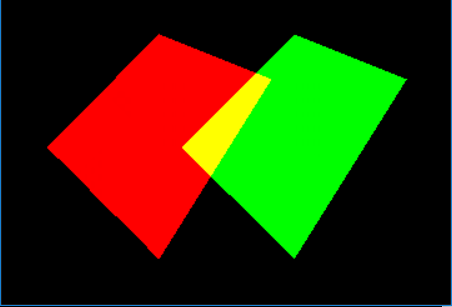
\includegraphics[height=3.5in, width = 3.7in]{images/without2}
    & 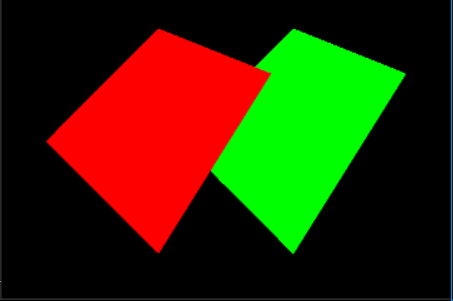
\includegraphics[height=3.5in, width = 3.7in]{images/with02}
    \\ (a) rendered without proposed method & (b) rendered with proposed algorithm
    \end{array}$
\end{center}
\caption{Results of proposed method implementation for two intersecting rectangles with different depth (red one being closest) } \label{fig:comparison1} 
\end{figure*}
    
\begin{figure*}[t]
\begin{center}
    $\begin{array}{@{\hspace{-0.00in}}c@{\hspace{0.05in}}c}
    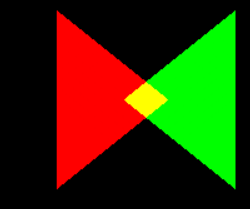
\includegraphics[height=3.07in]{images/without}
    & 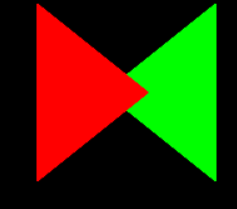
\includegraphics[height=3.07in]{images/with3}
    \\ (a) rendered without proposed method & (b) rendered with proposed algorithm
    \end{array}$
\end{center}
\caption{Results of proposed method implementation for two intersecting triangles with different depth (red one being closest) } \label{fig:comparison2} 
\end{figure*}
    
    
\begin{figure*}[t]
\begin{center}
    $\begin{array}{@{\hspace{-0.00in}}c@{\hspace{0.05in}}c}
    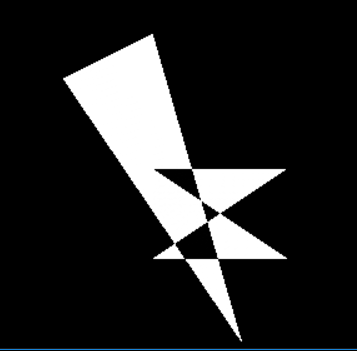
\includegraphics[height=3.5in]{images/withoutallwhite}
    & 
\includegraphics[height=3.5in]{images/withallwhite}
     \\ (a) rendered without proposed method & (b) rendered with proposed algorithm
    \end{array}$
\end{center}
\caption{Results of proposed method implementation for two monochrome intersecting shapes with different depth } \label{fig:comparison3} 
\end{figure*}

\begin{figure*}[t]
\begin{center}
    $\begin{array}{@{\hspace{-0.05in}}c@{\hspace{0.05in}}c@{\hspace{0.05in}}c}
    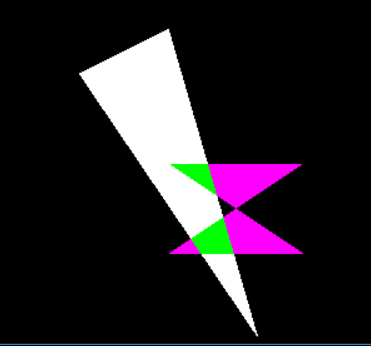
\includegraphics[height=2.07in]{images/without5}
    &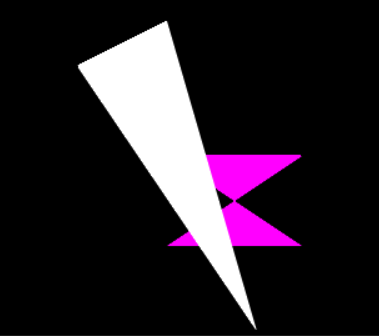
\includegraphics[height=2.07in]{images/with5pb}
     &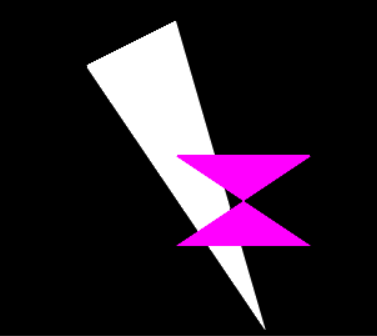
\includegraphics[height=2.07in]{images/withpinfront}
   \\ (a) without proposed method & (b) with proposed algorithm  &(c) with proposed algorithm 
    \end{array}$
\end{center}
\caption{Results of proposed method implementation for two intersecting shapes with different depth (a)without proposed method magenta shape behind (b) with proposed algorithm magenta shape in front  } \label{fig:comparison4} 

\end{figure*}

All shapes are rendered with scanline conversion without depth test. Clipping algorithm works very effectively to clip away part of the polygons that are not on the particular scanline and also to clip off of each polygons the piece that is inside a pixel. With a sorted z list for all pieces of polygons lying on a particular pixel, it can determine visible part of each pieces thus eliminating completely occluded polygons pieces. Pixel intensity is then area weighted average intensities which blurs the jagged edges giving the smooth illusion. If we look at Figure ~\ref{fig:comparison1} and ~\ref{fig:comparison2}, we can observe this blurred effect along the edges of rectangles and triangles. Also, in pixels with intersecting polygons, red (farthest polygon's color) doesn't show through when it's completely occluded by the green, otherwise red and green color is weighted by their respective area inside that particular pixel. In figure ~\ref{fig:comparison3}, after eliminating aliasing effect, edges look very nice without any saw tooth effect like before. Implementation of this algorithm works perfectly for removing hidden surfaces of irregular shapes as well (Figure ~\ref{fig:comparison4}). 

%\fontsize{8pt}{8pt}\selectfont
%\itemsep 0.0in
%\parskip 0.03in
%\parsep 2pt


\bibliographystyle{acmsiggraph}
\nocite{*}
\bibliography{symmetry}
\end{document}
